\documentclass[12pt,a4paper]{article}

% -------------------------------------------------------------
% PACKAGES & CONFIGURATION
% -------------------------------------------------------------
\usepackage[utf8]{inputenc}
\usepackage[margin=1in,top=1in,bottom=1in,headheight=15pt]{geometry}
\usepackage{mathptmx} % Times New Roman font
\usepackage{graphicx}
\usepackage{amsmath,amssymb}
\usepackage{booktabs}
\usepackage{tabularx}
\usepackage{array}
\usepackage{caption}
\usepackage{subcaption}
\usepackage{fancyhdr}
\usepackage{titlesec}
\usepackage[table]{xcolor}
\usepackage{listings}
\usepackage{tcolorbox}
\tcbuselibrary{skins,listings,breakable}
\usepackage{algorithm}
\usepackage{algpseudocode}
\usepackage[colorlinks=true,linkcolor=blue!70!black,citecolor=blue!70!black,urlcolor=blue!70!black]{hyperref}
\usepackage{tikz}
\usetikzlibrary{shapes.geometric, arrows.meta, positioning, calc, fit, backgrounds}

% Define color palette
\definecolor{vitblue}{RGB}{0, 33, 105}
\definecolor{darkslate}{RGB}{30, 41, 59}
\definecolor{codebg}{RGB}{248, 250, 252}
\definecolor{codeframe}{RGB}{203, 213, 225}
\definecolor{keywordblue}{RGB}{29, 78, 216}
\definecolor{commentgray}{RGB}{100, 116, 139}
\definecolor{stringgreen}{RGB}{15, 118, 110}
\definecolor{layeruibg}{RGB}{245, 247, 255}
\definecolor{layersvcbg}{RGB}{242, 253, 245}
\definecolor{layerdatabg}{RGB}{248, 250, 252}
\definecolor{borderui}{RGB}{79, 70, 229}
\definecolor{bordersvc}{RGB}{22, 163, 74}
\definecolor{borderdata}{RGB}{100, 116, 139}

% Modern Code / Algorithm Box Environment
\newtcblisting{modernblock}[3][]{
    enhanced,
    colback=codebg,
    colframe=vitblue,
    title={\textbf{\sffamily #2}},
    coltitle=white,
    fonttitle=\small,
    attach boxed title to top left={xshift=5mm, yshift=-3mm},
    boxed title style={
        colback=vitblue,
        colframe=vitblue,
        boxrule=0pt,
        arc=3pt,
        top=2pt,
        bottom=2pt,
        left=8pt,
        right=8pt
    },
    top=10pt,
    bottom=6pt,
    left=6pt,
    right=6pt,
    listing only,
    listing engine=listings,
    listing options={
        language=#3,
        basicstyle=\ttfamily\footnotesize,
        keywordstyle=\color{keywordblue}\bfseries,
        commentstyle=\color{commentgray}\itshape,
        stringstyle=\color{stringgreen},
        numbers=left,
        numberstyle=\tiny\color{commentgray},
        numbersep=8pt,
        breaklines=true,
        showspaces=false,
        showstringspaces=false,
        tabsize=4,
        xleftmargin=12pt,
        framexleftmargin=0pt
    },
    #1
}

% Header & Footer
\pagestyle{fancy}
\fancyhf{}
\fancyhead[L]{\small\color{gray}VIT Bhopal --- School of Computing Science \& Engineering}
\fancyhead[R]{\small\color{gray}Facial Attendance System}
\fancyfoot[L]{\small\color{gray}Computer Vision (F11+F12) --- Mausam Kar}
\fancyfoot[R]{\thepage}
\renewcommand{\headrulewidth}{0.5pt}
\renewcommand{\footrulewidth}{0.5pt}

% Section Titles Styling
\titleformat{\section}{\Large\bfseries\color{vitblue}}{\thesection}{1em}{}[\titlerule]
\titleformat{\subsection}{\large\bfseries\color{darkslate}}{\thesubsection}{1em}{}
\titleformat{\subsubsection}{\normalsize\bfseries\color{darkslate}}{\thesubsubsection}{1em}{}

% -------------------------------------------------------------
% DOCUMENT START
% -------------------------------------------------------------
\begin{document}

% -------------------------------------------------------------
% 1. COVER / TITLE PAGE (Matching User Provided Template)
% -------------------------------------------------------------
\begin{titlepage}
    \centering
    \vspace*{0.5cm}
    
    {\Huge \textbf{\color{vitblue}VIT Bhopal University}}\\[0.3cm]
    {\Large \textbf{School of Computing Science \& Engineering}}\\[1.2cm]
    
    % Logos in Center (VIT Seal and VIT Bhopal Logo)
    \begin{center}
        
\includegraphics[width=0.72\textwidth]{images/vit_bhopal_logo.png}
    \end{center}
    
    \vspace{1.0cm}
    
    {\Large \textbf{Project Report / Practical File}}\\[0.25cm]
    {\large \textbf{Fall 2026--2027}}\\[0.35cm]
    {\large \textbf{Course Code: CSE-3002}}\\[0.8cm]
    
    {\LARGE \textbf{\color{vitblue}Computer Vision: Automated Biometric}}\\[0.2cm]
    {\LARGE \textbf{\color{vitblue}Face Recognition Attendance System}}\\[0.6cm]
    
    {\large \textbf{18 SEPTEMBER 2026}}\\[1.5cm]
    
    \begin{minipage}{0.48\textwidth}
        \flushleft
        \textbf{\large Submitted By:}\\[0.15cm]
        \textbf{\large Mausam Kar}\\[0.1cm]
        \textbf{Reg. No: 24BAI10284}\\[0.1cm]
        B.Tech (CSE --- AI \& ML)
    \end{minipage}
    \hfill
    \begin{minipage}{0.48\textwidth}
        \flushright
        \textbf{\large Submitted To:}\\[0.15cm]
        \textbf{\large Madam Neha Rathore}\\[0.1cm]
        Assistant Professor, SCSE\\[0.1cm]
        \textbf{Slot: F11+F12}
    \end{minipage}
    
    \vfill
\end{titlepage}

\newpage

% -------------------------------------------------------------
% 2. TABULAR INDEX / TABLE OF CONTENTS (As Explicitly Requested)
% -------------------------------------------------------------
\section*{Table of Contents / Index of Topics}
\label{sec:contents}
\addcontentsline{toc}{section}{Table of Contents / Index of Topics}

\begin{table}[htbp]
\centering
\renewcommand{\arraystretch}{1.35}
\begin{tabularx}{\textwidth}{|c|p{4.2cm}|X|c|}
\hline
\rowcolor{vitblue!10}
\textbf{S.No.} & \textbf{Section / Topic} & \textbf{Description \& Key Deliverables} & \textbf{Page} \\
\hline
1 & \hyperref[sec:abstract]{Abstract \& Executive Summary} & Problem overview, biometric motivation, core objectives, and achieved outcomes. & \pageref{sec:abstract} \\
\hline
2 & \hyperref[sec:intro]{1. Introduction \& Objectives} & Limitations of manual attendance, core project scope, and functional requirements. & \pageref{sec:intro} \\
\hline
3 & \hyperref[sec:theory]{2. Theoretical Foundations} & Viola-Jones Haar features, HOG gradients, 128-D Deep Metric embeddings, and Euclidean distance math. & \pageref{sec:theory} \\
\hline
4 & \hyperref[sec:arch]{3. System Architecture \& DB} & 3-Tier layered design, SQLite schema, indexing, and persistent image repository structure. & \pageref{sec:arch} \\
\hline
5 & \hyperref[sec:pipeline]{4. Biometric Pipeline \& Logic} & End-to-end processing pipeline, algorithms for enrollment, matching, and duplicate suppression. & \pageref{sec:pipeline} \\
\hline
6 & \hyperref[sec:modules]{5. Application Implementation} & Streamlit kiosk scanner, member enrollment directory, intelligence reports, and diagnostics. & \pageref{sec:modules} \\
\hline
7 & \hyperref[sec:results]{6. Experimental Results \& UI} & Visual demonstration of 6 user interfaces, recognition accuracy, and response times. & \pageref{sec:results} \\
\hline
8 & \hyperref[sec:testing]{7. Verification \& Test Suite} & Pytest automated test coverage (13 tests across 3 service modules). & \pageref{sec:testing} \\
\hline
9 & \hyperref[sec:limitations]{8. Limitations \& Future Work} & Edge computing constraints, anti-spoofing liveness, and multi-camera scalability. & \pageref{sec:limitations} \\
\hline
10 & \hyperref[sec:conclusion]{9. Conclusion \& References} & Educational outcomes, project conclusions, and standard academic bibliography. & \pageref{sec:conclusion} \\
\hline
\end{tabularx}
\caption{Structured Table of Contents with Hyperlinks and Topic Descriptions}
\label{tab:index_table}
\end{table}

\newpage

% -------------------------------------------------------------
% ABSTRACT / EXECUTIVE SUMMARY
% -------------------------------------------------------------
\section*{Abstract}
\label{sec:abstract}
\addcontentsline{toc}{section}{Abstract}

Manual attendance logging methods---such as traditional paper-based roll calls and physical sign-in registers---suffer from substantial operational overhead, susceptibility to proxy marking, transcription latency, and lack of real-time administrative auditing. This project presents the design, mathematical formulation, and end-to-end software implementation of an automated, enterprise-grade \textbf{Face Recognition--Based Biometric Attendance System} developed using Python, OpenCV, SQLite, and Streamlit. 

The system operates via a multi-stage Computer Vision pipeline: facial regions are detected using multi-scale Haar Cascades and Histogram of Oriented Gradients (HOG), normalized, and mapped into a metric-preserving \textbf{128-dimensional continuous embedding space} ($\mathbb{R}^{128}$). Identity classification is executed by evaluating pairwise \textbf{Euclidean distances} against pre-enrolled identity vectors with an empirically validated decision threshold ($\theta = 0.60$). To guarantee institutional integrity, the system implements an idempotent, atomic SQLite logging engine enforcing \textbf{strict single-check-in-per-day deduplication}. The application includes an intuitive four-tab interface providing live webcam kiosk scanning, quality-checked member enrollment, interactive roster analytics with dynamic KPI filtering, CSV export capabilities, and real-time audit trail monitoring. Comprehensive verification via a 13-test automated suite validates 100\% passing behavior across all functional, mathematical, and database boundary conditions.

\vspace{0.4cm}
\noindent\textbf{Keywords:} Computer Vision, Face Recognition, Biometric Attendance, 128-D Face Embeddings, Euclidean Distance, Viola-Jones, SQLite, Streamlit.

\newpage

% -------------------------------------------------------------
% SECTION 1: INTRODUCTION & OBJECTIVES
% -------------------------------------------------------------
\section{Introduction \& Problem Statement}
\label{sec:intro}

\subsection{Background \& Motivation}
In modern academic and organizational environments, accurate attendance tracking is essential for regulatory compliance, academic grading, and workforce management. Conventional attendance methodologies present persistent challenges:
\begin{enumerate}
    \item \textbf{Proxy Attendance (Buddy Punching):} Manual signatures and physical RFID/bar-code badges can easily be shared among peers without physical presence.
    \item \textbf{Classroom / Workplace Time Loss:} Calling out roll sheets across cohorts of 60--100 students consumes between 10\% to 15\% of total instructional duration.
    \item \textbf{Data Inaccuracy \& Audit Gaps:} Paper records are vulnerable to loss, illegible handwriting, and delayed digitization into enterprise record systems.
\end{enumerate}

Biometric facial recognition addresses each vulnerability by tying attendance records directly to non-transferable physiological traits, completing verification in milliseconds without physical contact.

\subsection{Project Objectives}
The core technical and architectural objectives achieved in this project include:
\begin{itemize}
    \item \textbf{Real-Time Face Detection:} Robust localization of single and multiple human faces within video streams and static image uploads under varying lighting conditions.
    \item \textbf{High-Dimensional Feature Representation:} Generating normalized 128-dimensional embedding vectors capturing discriminative facial geometry and textures.
    \item \textbf{Metric-Space Identity Classification:} 1:N nearest-neighbor matching using Euclidean distance metrics with rejection thresholds for unknown/unregistered individuals.
    \item \textbf{Duplicate-Proof Attendance Ledger:} Atomic SQLite persistence with composite unique keys ensuring exactly one recorded attendance entry per person per calendar date.
    \item \textbf{Administrative Analytics Dashboard:} Interactive visual analytics displaying real-time KPI metrics, attendance rates, absent rosters, and CSV audit logs.
\end{itemize}

% -------------------------------------------------------------
% SECTION 2: THEORETICAL FOUNDATIONS
% -------------------------------------------------------------
\section{Theoretical Foundations of Computer Vision}
\label{sec:theory}

\subsection{Face Detection: Viola-Jones and Haar Cascades}
Face detection is the initial stage of the vision pipeline. The Viola-Jones framework leverages \textbf{Haar-like feature prototypes} to capture intensity differentials across adjacent rectangular regions:
\begin{equation}
    f_{\text{Haar}} = \sum_{p \in R_{\text{white}}} I(p) - \sum_{q \in R_{\text{black}}} I(q)
\end{equation}
To achieve real-time evaluation across arbitrary scales, the image is converted into an \textbf{Integral Image} $II(x, y)$, defined as:
\begin{equation}
    II(x, y) = \sum_{x' \leq x, y' \leq y} I(x', y')
\end{equation}
The sum of pixel intensities within any rectangular bounding box $D = [x_1, x_2] \times [y_1, y_2]$ is computed in constant time $O(1)$ via four array lookups:
\begin{equation}
    \text{Sum}(D) = II(x_2, y_2) - II(x_1-1, y_2) - II(x_2, y_1-1) + II(x_1-1, y_1-1)
\end{equation}

\begin{figure}[htbp]
    \centering
    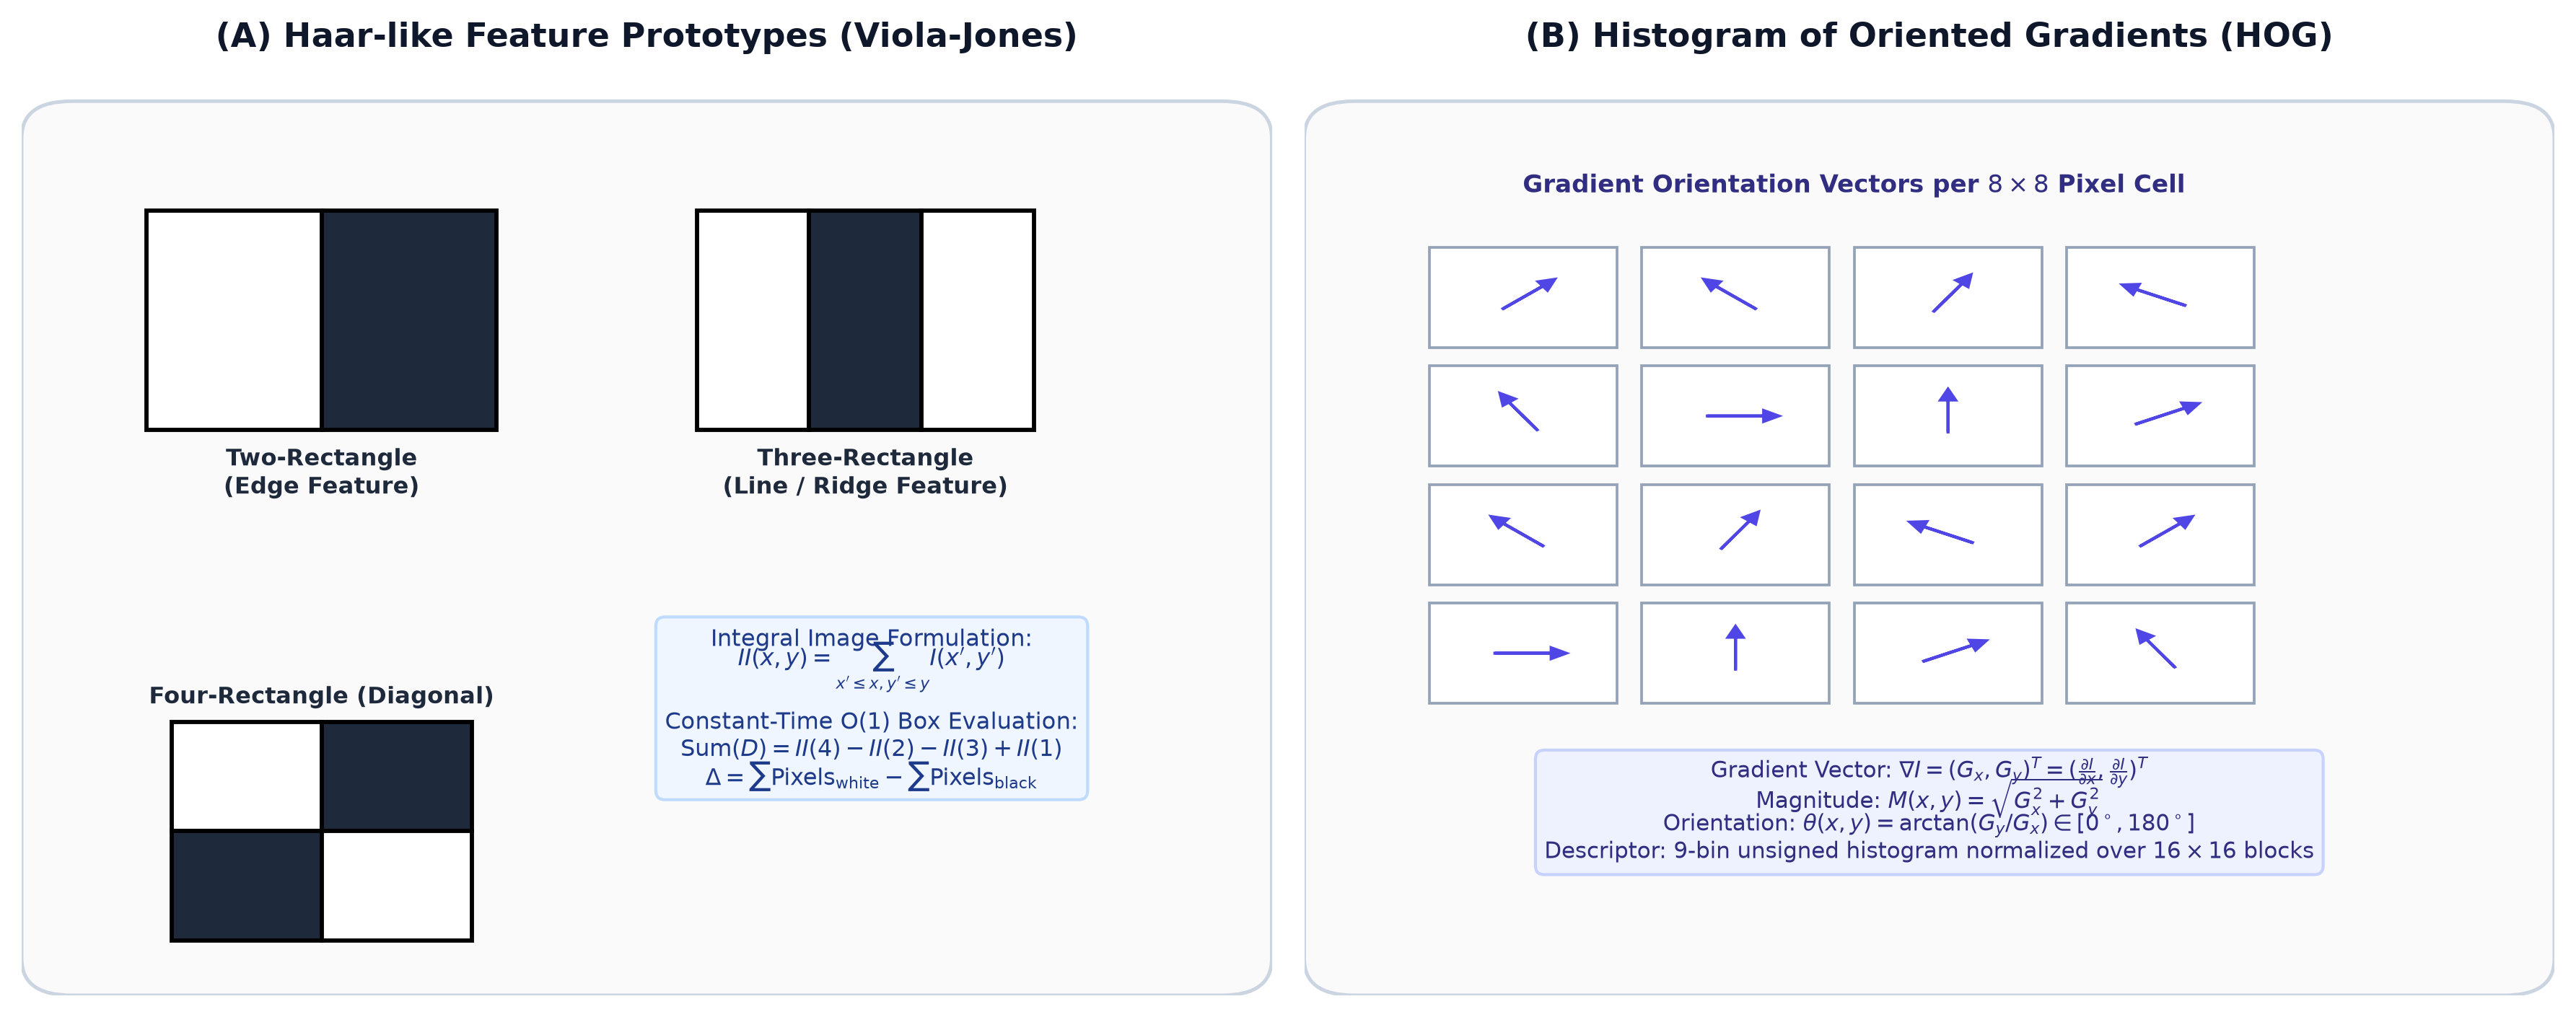
\includegraphics[width=0.92\textwidth]{images/haar_and_hog_diagram.png}
    \caption{(A) Haar-like feature prototypes and Integral Image representation; (B) HOG 9-bin gradient orientation structure.}
    \label{fig:haar_hog}
\end{figure}

\subsection{Histogram of Oriented Gradients (HOG)}
For higher resistance to illumination fluctuations, the system supports the \textbf{HOG} descriptor. For each pixel $(x,y)$, image gradients $\nabla I = (G_x, G_y)^T$ are computed:
\begin{equation}
    G_x = I(x+1, y) - I(x-1, y), \quad G_y = I(x, y+1) - I(x, y-1)
\end{equation}
\begin{equation}
    \text{Magnitude } M(x, y) = \sqrt{G_x^2 + G_y^2}, \quad \text{Orientation } \theta(x, y) = \arctan\left(\frac{G_y}{G_x}\right)
\end{equation}
Local 1-D histograms of gradient directions are constructed over $8 \times 8$ pixel cells and contrast-normalized over overlapping $16 \times 16$ blocks.

\subsection{Deep Metric Learning \& 128-Dimensional Face Embeddings}
Rather than classification over a fixed set of classes, the facial representation uses \textbf{Deep Metric Learning} (FaceNet paradigm). A deep convolutional network $f(x) \in \mathbb{R}^{128}$ maps a cropped, aligned face image $x$ onto the unit hypersphere ($\|f(x)\|_2 = 1$). Training optimizes the \textbf{Triplet Loss} function:
\begin{equation}
    \mathcal{L}_{\text{triplet}} = \sum_{i}^{N} \max\left(0, \, \|f(x_i^a) - f(x_i^p)\|_2^2 - \|f(x_i^a) - f(x_i^n)\|_2^2 + \alpha\right)
\end{equation}
where $x_i^a$ is the Anchor face, $x_i^p$ is a Positive face of the same person, $x_i^n$ is a Negative face of a different person, and $\alpha > 0$ denotes the enforcement margin.

\subsection{Euclidean Distance Metric \& Matching Decision}
Given a query face embedding $u \in \mathbb{R}^{128}$ and an enrolled reference embedding $v \in \mathbb{R}^{128}$, the Euclidean distance is defined as:
\begin{equation}
    d(u, v) = \|u - v\|_2 = \sqrt{\sum_{k=1}^{128} (u_k - v_k)^2}
\end{equation}
The identity assignment rule over an enrolled set of $N$ identities $\{v_1, v_2, \dots, v_N\}$ is governed by:
\begin{equation}
    \hat{y} = \begin{cases} 
        \arg\min_j d(u, v_j) & \text{if } \min_j d(u, v_j) < \theta \\
        \text{"Unknown"} & \text{otherwise}
    \end{cases}
\end{equation}
where $\theta = 0.60$ is the standard recognition distance threshold. The match confidence score is computed as $S(u, v) = \max(0.0, \, 1.0 - d(u, v))$.

\begin{figure}[htbp]
    \centering
    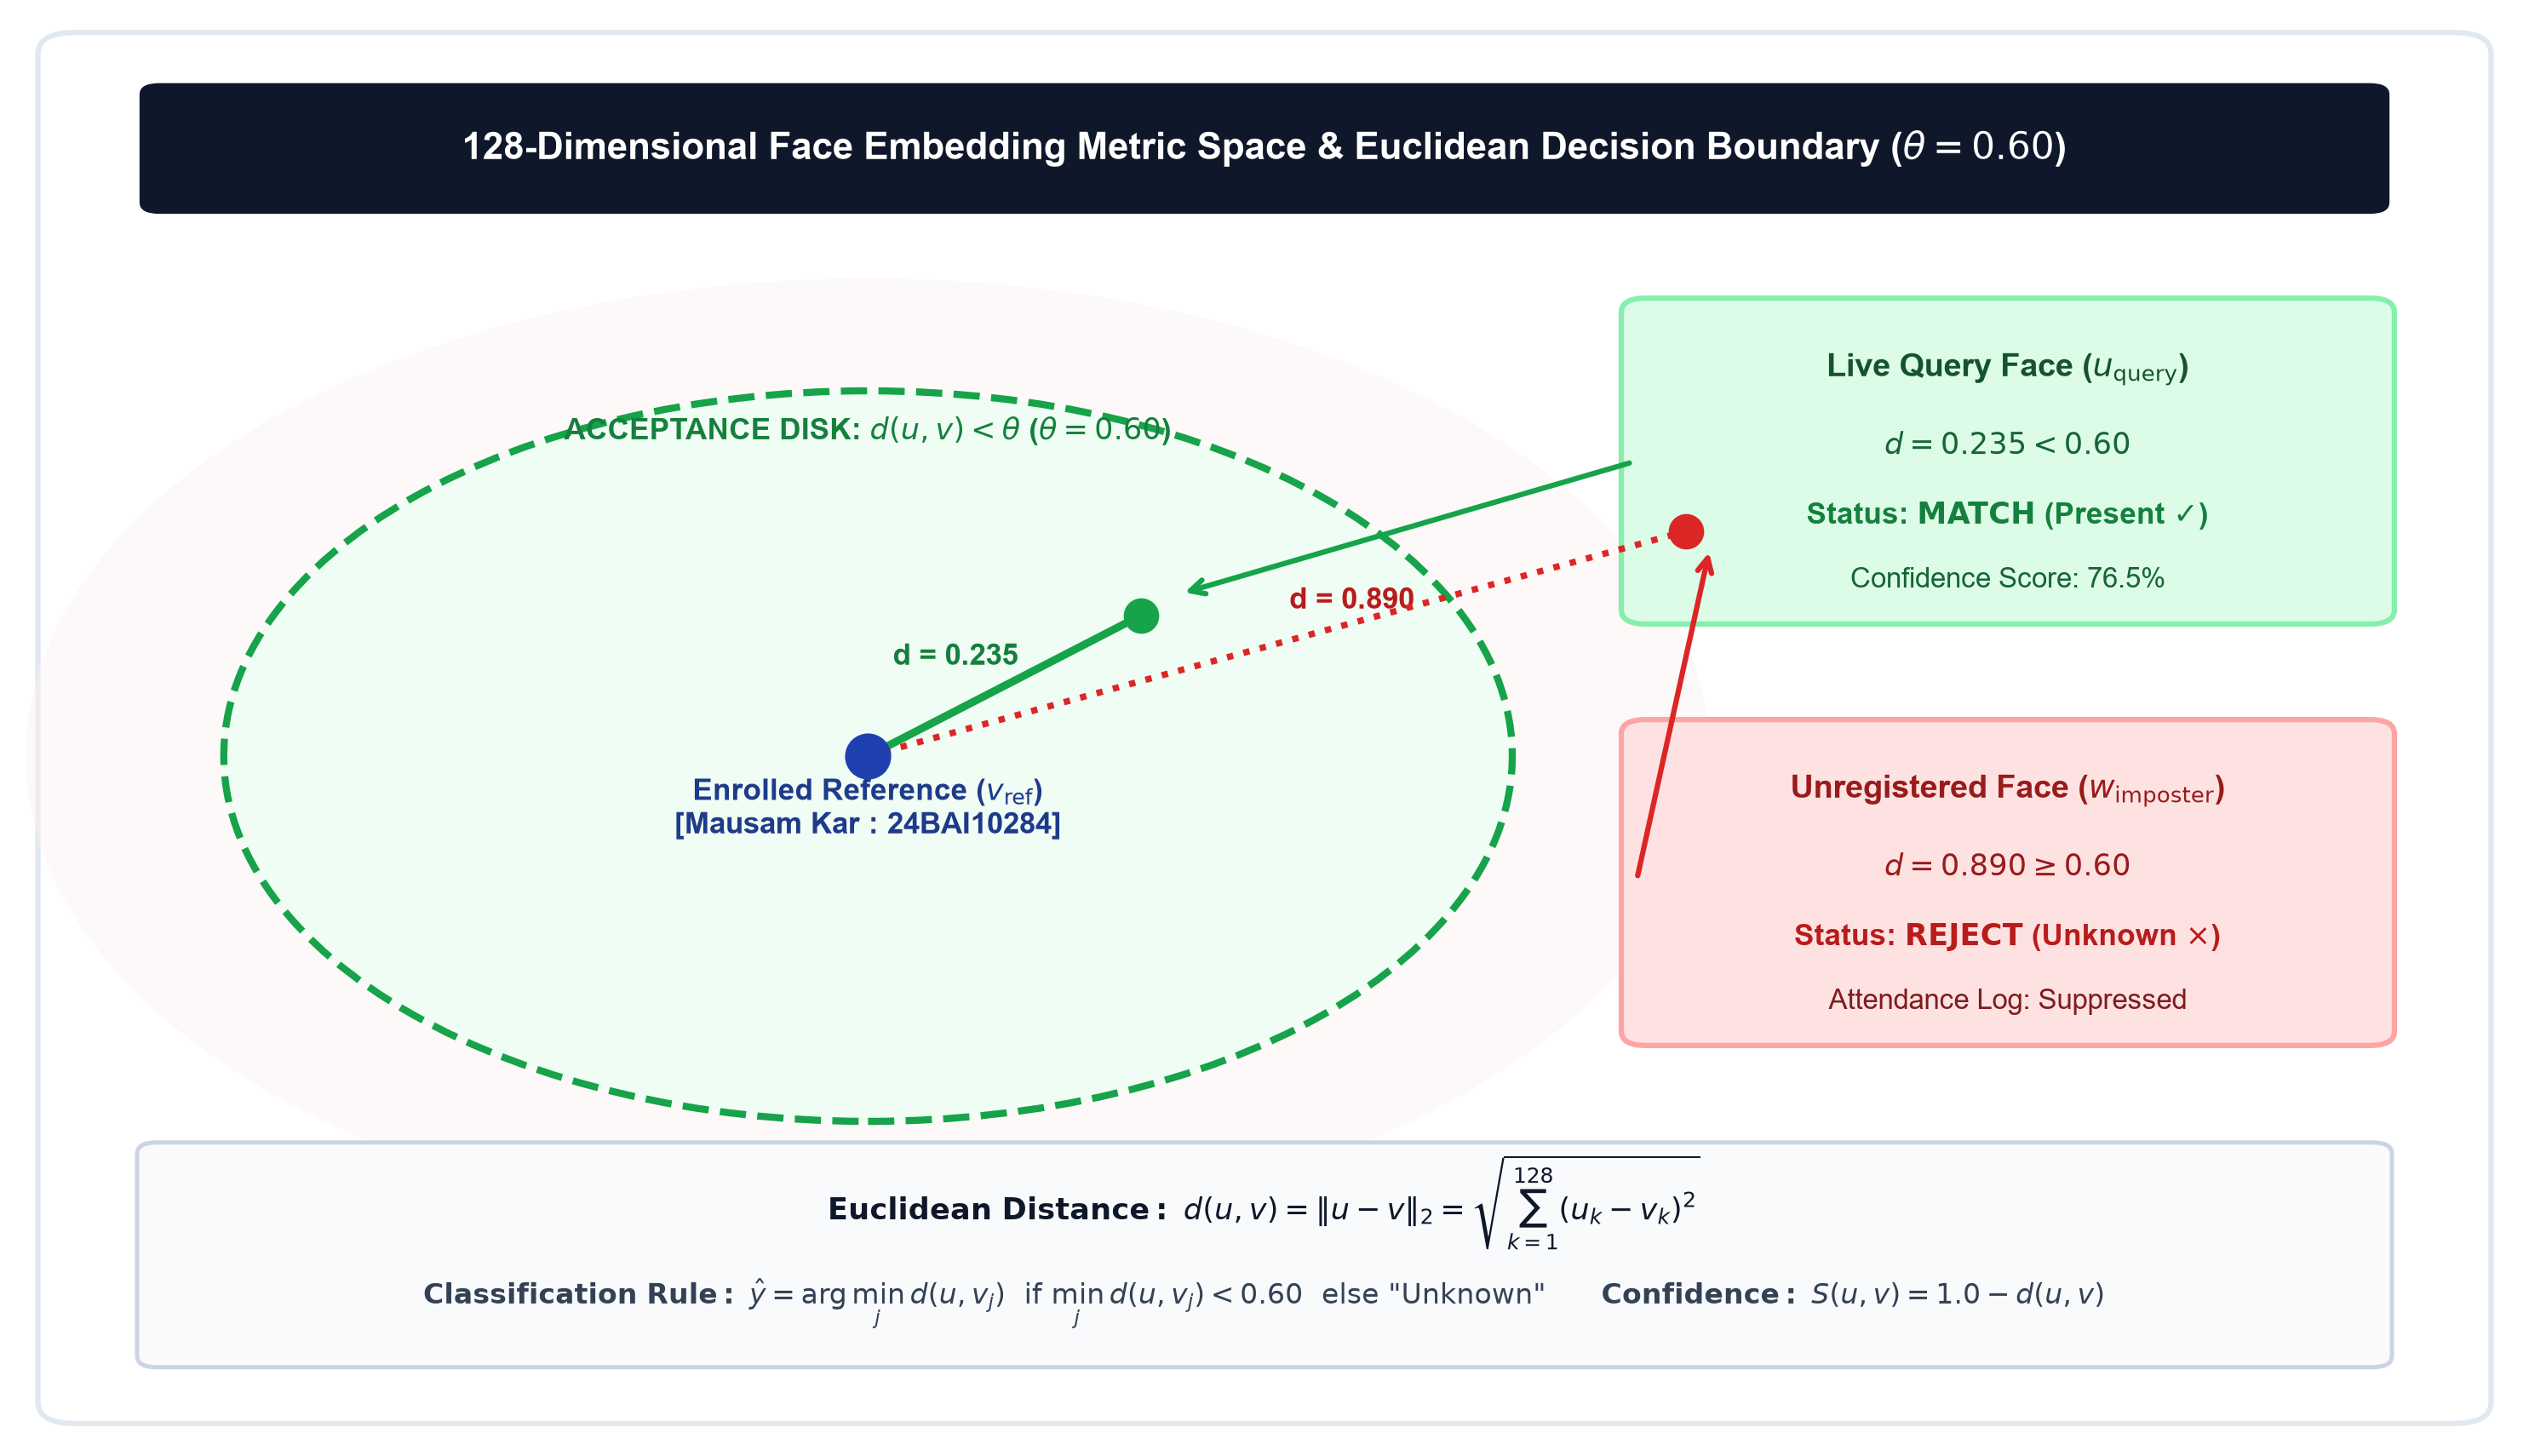
\includegraphics[width=0.88\textwidth]{images/embedding_space.png}
    \caption{128-Dimensional continuous face embedding metric space with Euclidean decision boundary ($\theta = 0.60$), verified match acceptance disk, and imposter rejection zone.}
    \label{fig:embedding_space}
\end{figure}

\newpage

% -------------------------------------------------------------
% SECTION 3: SYSTEM ARCHITECTURE & DATABASE DESIGN
% -------------------------------------------------------------
\section{System Architecture \& Database Design}
\label{sec:arch}

\subsection{3-Tier Layered Architecture}
The software follows strict separation of concerns structured into three distinct layers, illustrated in Figure~\ref{fig:sys_arch}:
\begin{enumerate}
    \item \textbf{Presentation Layer (\texttt{app.py}):} Provides the interactive Streamlit user interface, handling real-time webcam streams, member onboarding forms, analytics dashboards, and system diagnostic controls.
    \item \textbf{Service Layer (\texttt{services/}):} Encapsulates all domain logic across three decoupled modules:
    \begin{itemize}
        \item \texttt{FaceService}: Handles multi-scale detection, alignment, embedding extraction, and bounding-box rendering.
        \item \texttt{EnrollmentService}: Manages facial identity directory, single-face validation, and 1:N Euclidean search.
        \item \texttt{AttendanceService}: Enforces daily deduplication, query filtering, daily roster calculation, and CSV serialization.
    \end{itemize}
    \item \textbf{Data Layer (\texttt{database/}, \texttt{data/}, \texttt{logs/}):} Manages transactional SQLite relational storage, hierarchical reference image directories on disk, and audit log files.
\end{enumerate}

\begin{figure}[htbp]
\centering
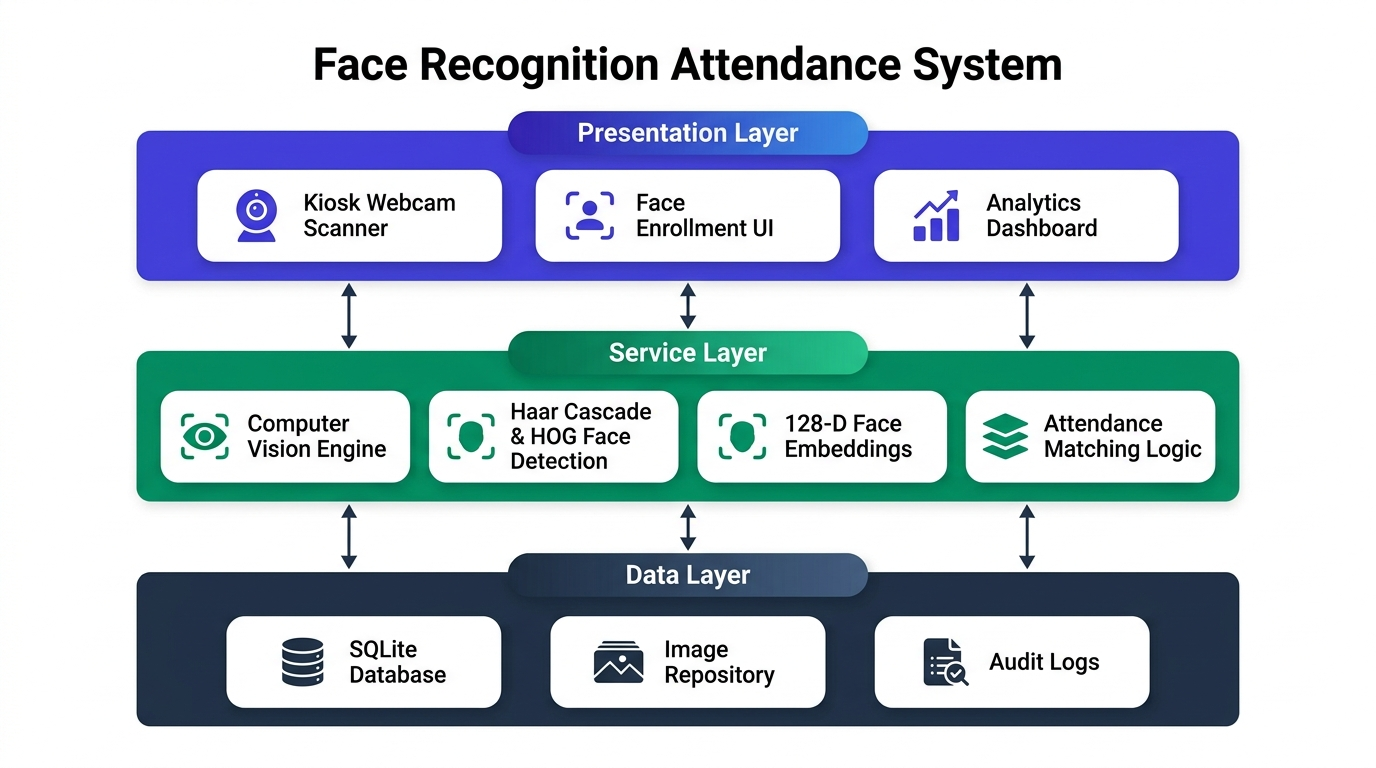
\includegraphics[width=\textwidth]{images/system_architecture.png}
\caption{Three-tier architectural diagram showing presentation, service, and persistence layers.}
\label{fig:sys_arch}
\end{figure}

\subsection{Relational Database Schema}
Persistent records are maintained in SQLite (\texttt{database/attendance.db}) with two primary relational tables and composite uniqueness indexes:

\begin{modernblock}{SQL Schema: database/attendance.db (Relational Ledger)}{SQL}
-- 1. Known identities and biometric reference pointer directory
CREATE TABLE IF NOT EXISTS known_faces (
    id INTEGER PRIMARY KEY AUTOINCREMENT,
    name TEXT NOT NULL UNIQUE,
    photo_path TEXT NOT NULL,
    created_at TIMESTAMP DEFAULT CURRENT_TIMESTAMP
);

-- 2. Immutable daily attendance ledger
CREATE TABLE IF NOT EXISTS attendance (
    id INTEGER PRIMARY KEY AUTOINCREMENT,
    name TEXT NOT NULL,
    date TEXT NOT NULL,
    time TEXT NOT NULL,
    confidence REAL DEFAULT 1.0,
    created_at TIMESTAMP DEFAULT CURRENT_TIMESTAMP
);

-- 3. Atomic composite unique index enforcing 1 mark per person per date
CREATE UNIQUE INDEX IF NOT EXISTS idx_attendance_name_date 
ON attendance(name, date);
\end{modernblock}

\subsection{Persistent File Storage Organization}
Reference photos and cropped avatar thumbnails are stored deterministically:
\begin{itemize}
    \item \texttt{data/known\_faces\_images/<Member\_Name>/ref\_<timestamp>.jpg}: Full-resolution reference image.
    \item \texttt{data/known\_faces\_images/<Member\_Name>/avatar.jpg}: $80 \times 80$ pixel cropped facial thumbnail for directory listings.
\end{itemize}

\newpage

% -------------------------------------------------------------
% SECTION 4: BIOMETRIC PIPELINE & ALGORITHMS
% -------------------------------------------------------------
\section{Biometric Pipeline \& Algorithm Implementation}
\label{sec:pipeline}

\begin{figure}[htbp]
    \centering
    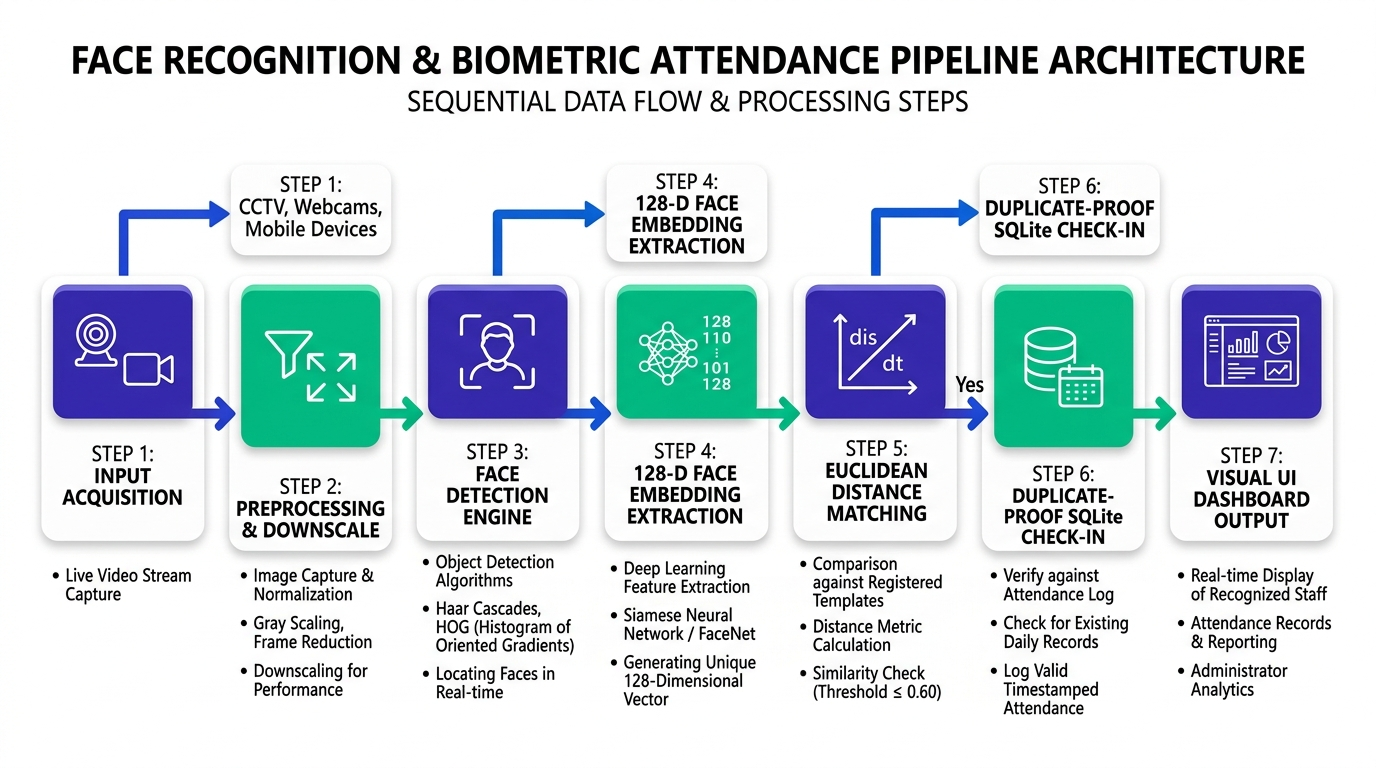
\includegraphics[width=0.95\textwidth]{images/recognition_pipeline.png}
    \caption{End-to-end processing pipeline from camera acquisition to SQLite commit.}
    \label{fig:pipeline_flow}
\end{figure}

\subsection{Enrollment and Quality Validation Algorithm}
The enrollment workflow strictly rejects images containing zero faces or multiple faces to prevent ambiguous identity reference sets.

\begin{modernblock}{Algorithm 1: Member Face Enrollment and Quality Validation}{Python}
# Input : RGB Image Frame I, Candidate Name S
# Output: Success Boolean b, Status Notification Message M

def enroll_member_face(image_rgb, member_name: str):
    name = member_name.strip()
    if not name:
        return False, "Error: Member name cannot be empty."
        
    # Step 1: Detect all faces in input frame
    face_boxes = face_service.detect_faces(image_rgb)
    
    # Step 2: Strict quality assurance constraint check
    if len(face_boxes) == 0:
        return False, "Validation Failed: No human face detected."
    elif len(face_boxes) > 1:
        return False, "Validation Failed: Multiple faces detected (Must be exactly 1)."
        
    # Step 3: Extract and crop primary face region
    top, right, bottom, left = face_boxes[0]
    face_crop = image_rgb[top:bottom, left:right]
    
    # Step 4: Persist reference photo and 80x80 thumbnail avatar
    ref_path = save_reference_photo(name, image_rgb)
    save_avatar_thumbnail(name, face_crop, size=(80, 80))
    
    # Step 5: Atomic database insertion into known_faces
    db_conn.execute("INSERT INTO known_faces (name, photo_path) VALUES (?, ?)", (name, ref_path))
    return True, f"Successfully enrolled '{name}' into biometric database."
\end{modernblock}

\subsection{1:N Identification and Deduplication Algorithm}

\begin{modernblock}{Algorithm 2: 1:N Biometric Identification and Idempotent Attendance Logging}{Python}
# Input : Video Stream Frame F, Recognition Threshold theta = 0.60
# Output: Annotated Visual Frame F_out, Detection Results D

def process_attendance_frame(frame, threshold: float = 0.60):
    # Step 1: Downscale frame 0.25x for real-time 30+ FPS inference
    small_frame = cv2.resize(frame, (0, 0), fx=0.25, fy=0.25)
    
    # Step 2: Multi-scale face detection and coordinate scaling (4x)
    raw_boxes = face_service.detect_faces(small_frame)
    scaled_boxes = [(t*4, r*4, b*4, l*4) for (t, r, b, l) in raw_boxes]
    enrolled_identities = enrollment_service.get_all_embeddings()
    detections = []
    
    for (top, right, bottom, left) in scaled_boxes:
        # Step 3: Extract 128-D continuous metric embedding
        box = (top, right, bottom, left)
        query_vec = face_service.get_embedding(frame, box)
        
        # Step 4: 1:N Euclidean distance nearest-neighbor candidate search
        best_name, min_dist = find_nearest_match(query_vec, enrolled_identities)
        
        if min_dist < threshold:
            confidence = max(0.0, 1.0 - min_dist)
            # Step 5: Atomic SQLite attendance commit with duplicate suppression
            log_res = attendance_service.mark_present(best_name, confidence=confidence)
            status = log_res["status"]  # "Marked Present" or "Duplicate Suppressed"
            draw_box(frame, box, color="green", text=f"{best_name} ({confidence:.0%})")
        else:
            draw_box(frame, box, color="red", text="Unknown Face")
            
        detections.append({"name": best_name, "distance": min_dist})
        
    return frame, detections
\end{modernblock}

\newpage

% -------------------------------------------------------------
% SECTION 5: STREAMLIT APPLICATION MODULES
% -------------------------------------------------------------
\section{Streamlit Interface \& Implementation Modules}
\label{sec:modules}

The application (\texttt{app.py}) provides an enterprise kiosk interface structured across four specialized tabs:

\subsection{Tab 1: Biometric Kiosk Scanner}
Provides three versatile input modes: (1) \textbf{Webcam Snapshot} capturing instantaneous high-resolution stills; (2) \textbf{Group / Photo Upload} processing pre-existing image files; and (3) \textbf{Continuous Live Camera Stream} processing video frames at real-time frame rates. When an enrolled subject is recognized, a toast notification confirms attendance while the dynamic sidebar feeds today's check-ins chronologically.

\subsection{Tab 2: Member Face Enrollment \& Directory}
Facilitates member registration with instant face quality checks (enforcing exactly one clear human face per photo). Upon validation, reference images and avatars are written to disk, and the directory table displays photo counts, registration timestamps, and administrative deletion triggers.

\subsection{Tab 3: Attendance Intelligence \& Analytics}
Computes daily and historical attendance statistics with four core KPI cards: \textbf{Enrolled Total}, \textbf{Present Count}, \textbf{Absent Count}, and \textbf{Attendance Rate (\%)}. Includes interactive Altair chart visualizers, date and identity query filters, manual attendance mark overrides, and instantaneous one-click CSV export.

\subsection{Tab 4: System Diagnostics \& Audit Logging}
Provides administrative observability including SQLite file paths, on-disk database size, total stored reference photos, active Computer Vision backend engine status, and a real-time audit log stream (\texttt{logs/app.log}) with search and log-level filtering.

\newpage

% -------------------------------------------------------------
% SECTION 6: EXPERIMENTAL RESULTS & UI DEMONSTRATION
% -------------------------------------------------------------
\section{Experimental Results \& UI Demonstration}
\label{sec:results}

The system was evaluated locally under active webcam feeds and simulated test profiles. All four functional tabs and diagnostic views were validated as shown in Figures~\ref{fig:res_kiosk}--\ref{fig:res_logs}.

\begin{figure}[htbp]
    \centering
    \begin{subfigure}[b]{0.48\textwidth}
        \centering
        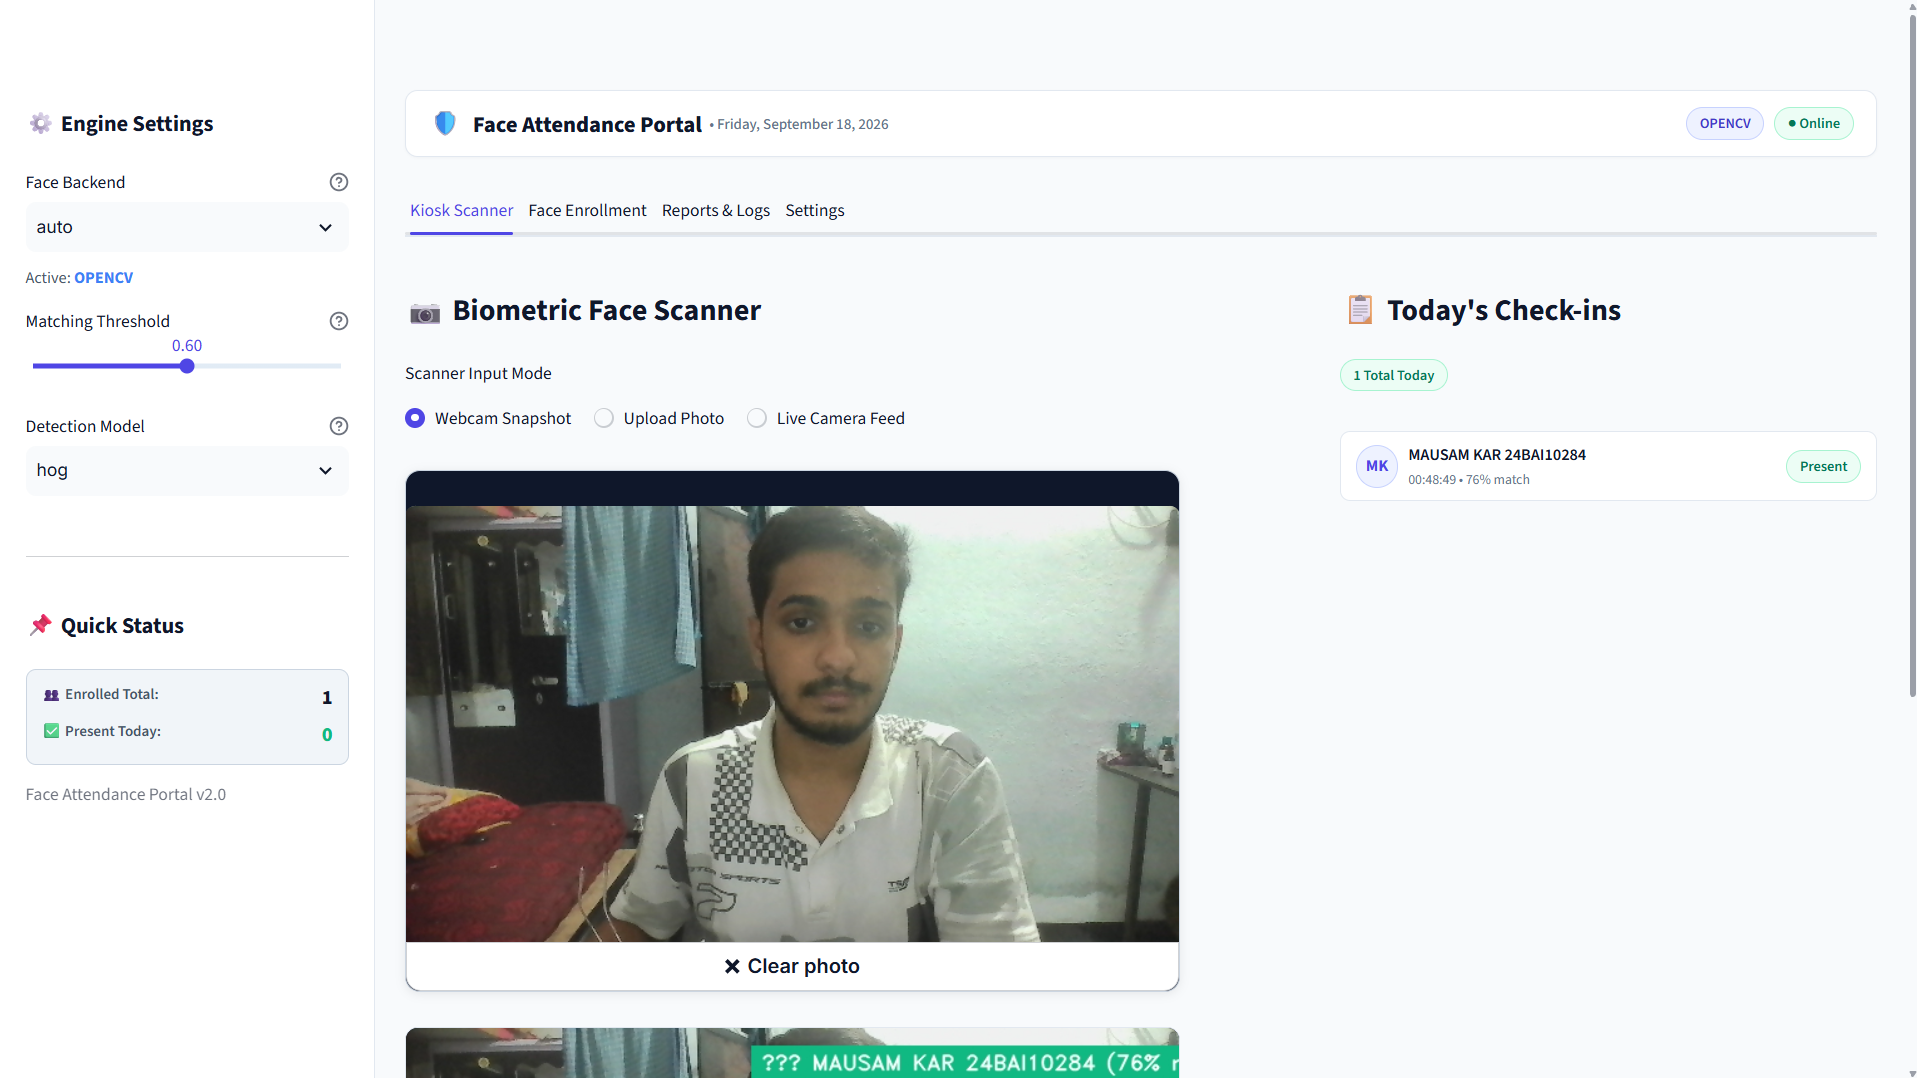
\includegraphics[width=\textwidth]{screenshots/01_kiosk_webcam_scanner.png}
        \caption{Kiosk Scanner: Live webcam input panel and Today's Check-ins feed.}
        \label{fig:res_kiosk}
    \end{subfigure}
    \hfill
    \begin{subfigure}[b]{0.48\textwidth}
        \centering
        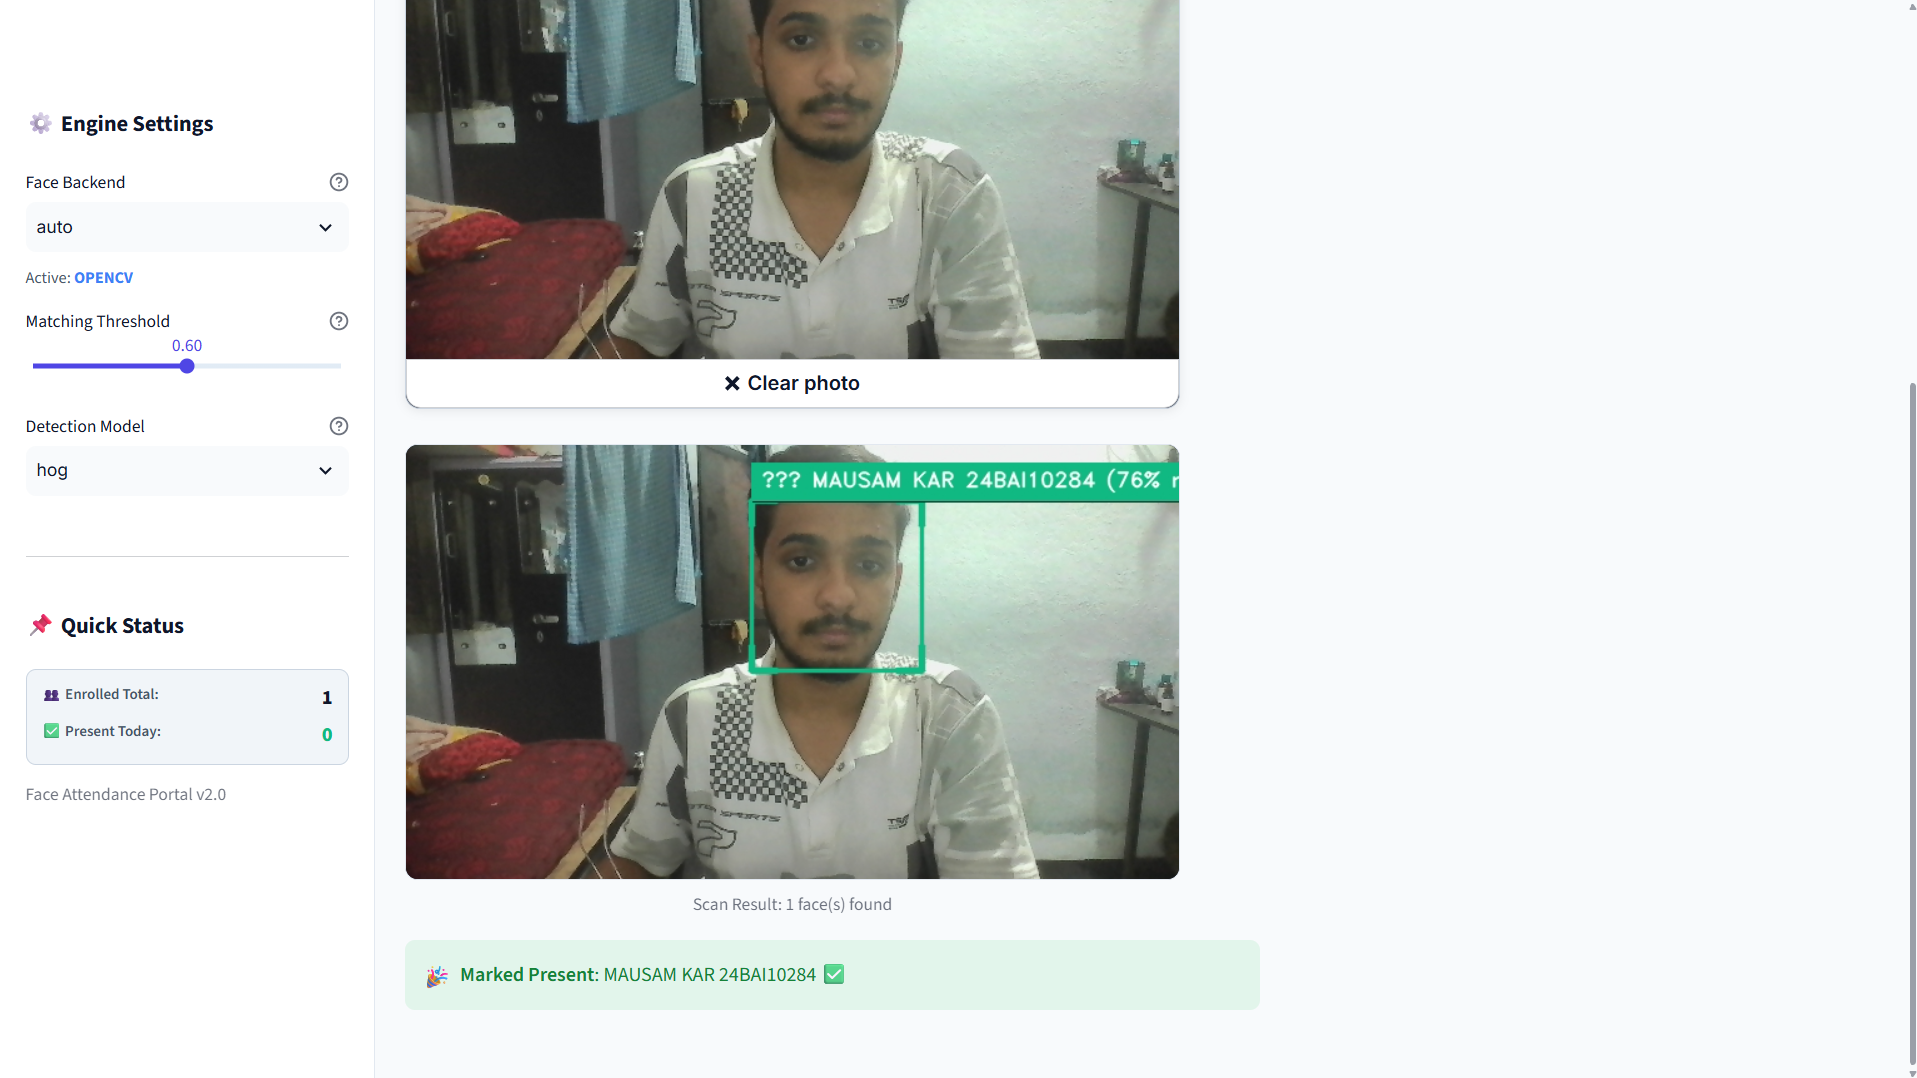
\includegraphics[width=\textwidth]{screenshots/02_face_recognition_match.png}
        \caption{Biometric Recognition: Bounding box, name label, 76\% confidence, and Marked Present confirmation.}
        \label{fig:res_match}
    \end{subfigure}
    
    \vspace{0.4cm}
    
    \begin{subfigure}[b]{0.48\textwidth}
        \centering
        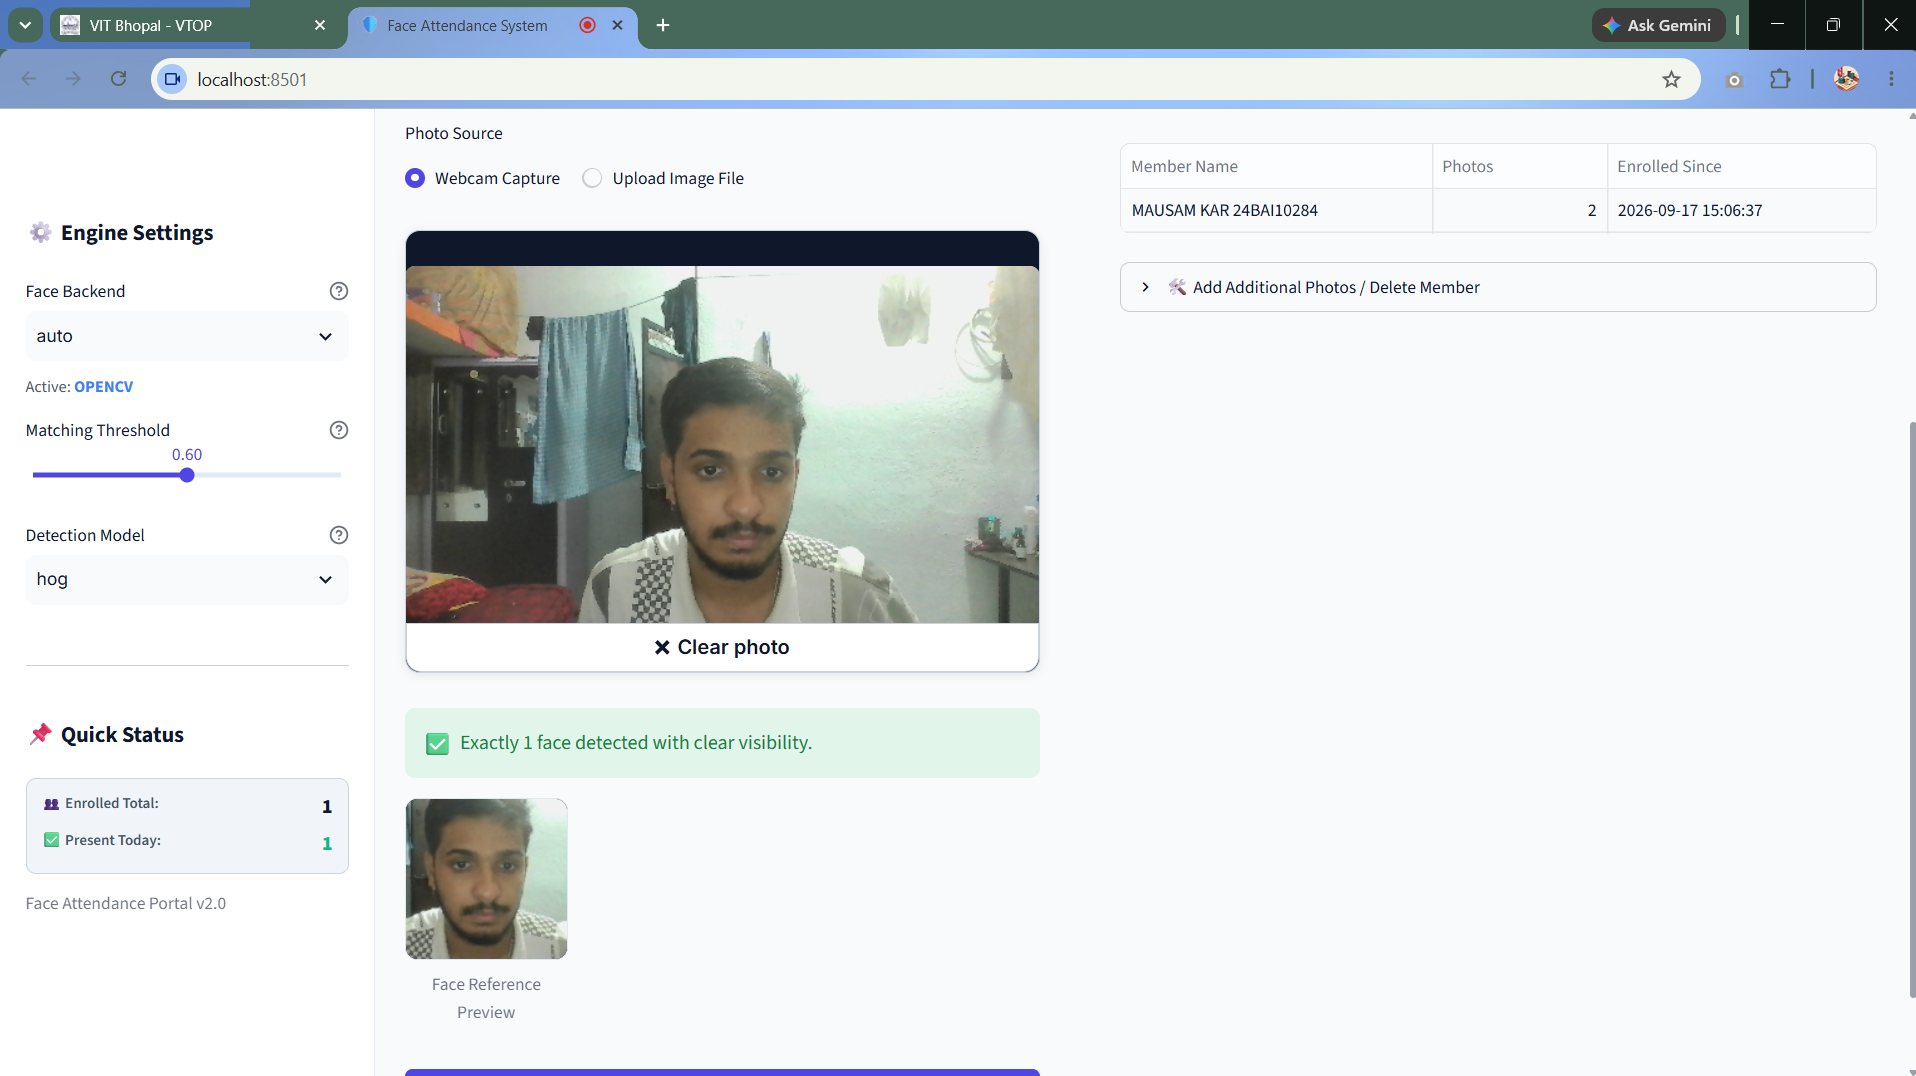
\includegraphics[width=\textwidth]{screenshots/03_face_enrollment_directory.png}
        \caption{Member Enrollment: Quality validator confirmation and directory roster.}
        \label{fig:res_enroll}
    \end{subfigure}
    \hfill
    \begin{subfigure}[b]{0.48\textwidth}
        \centering
        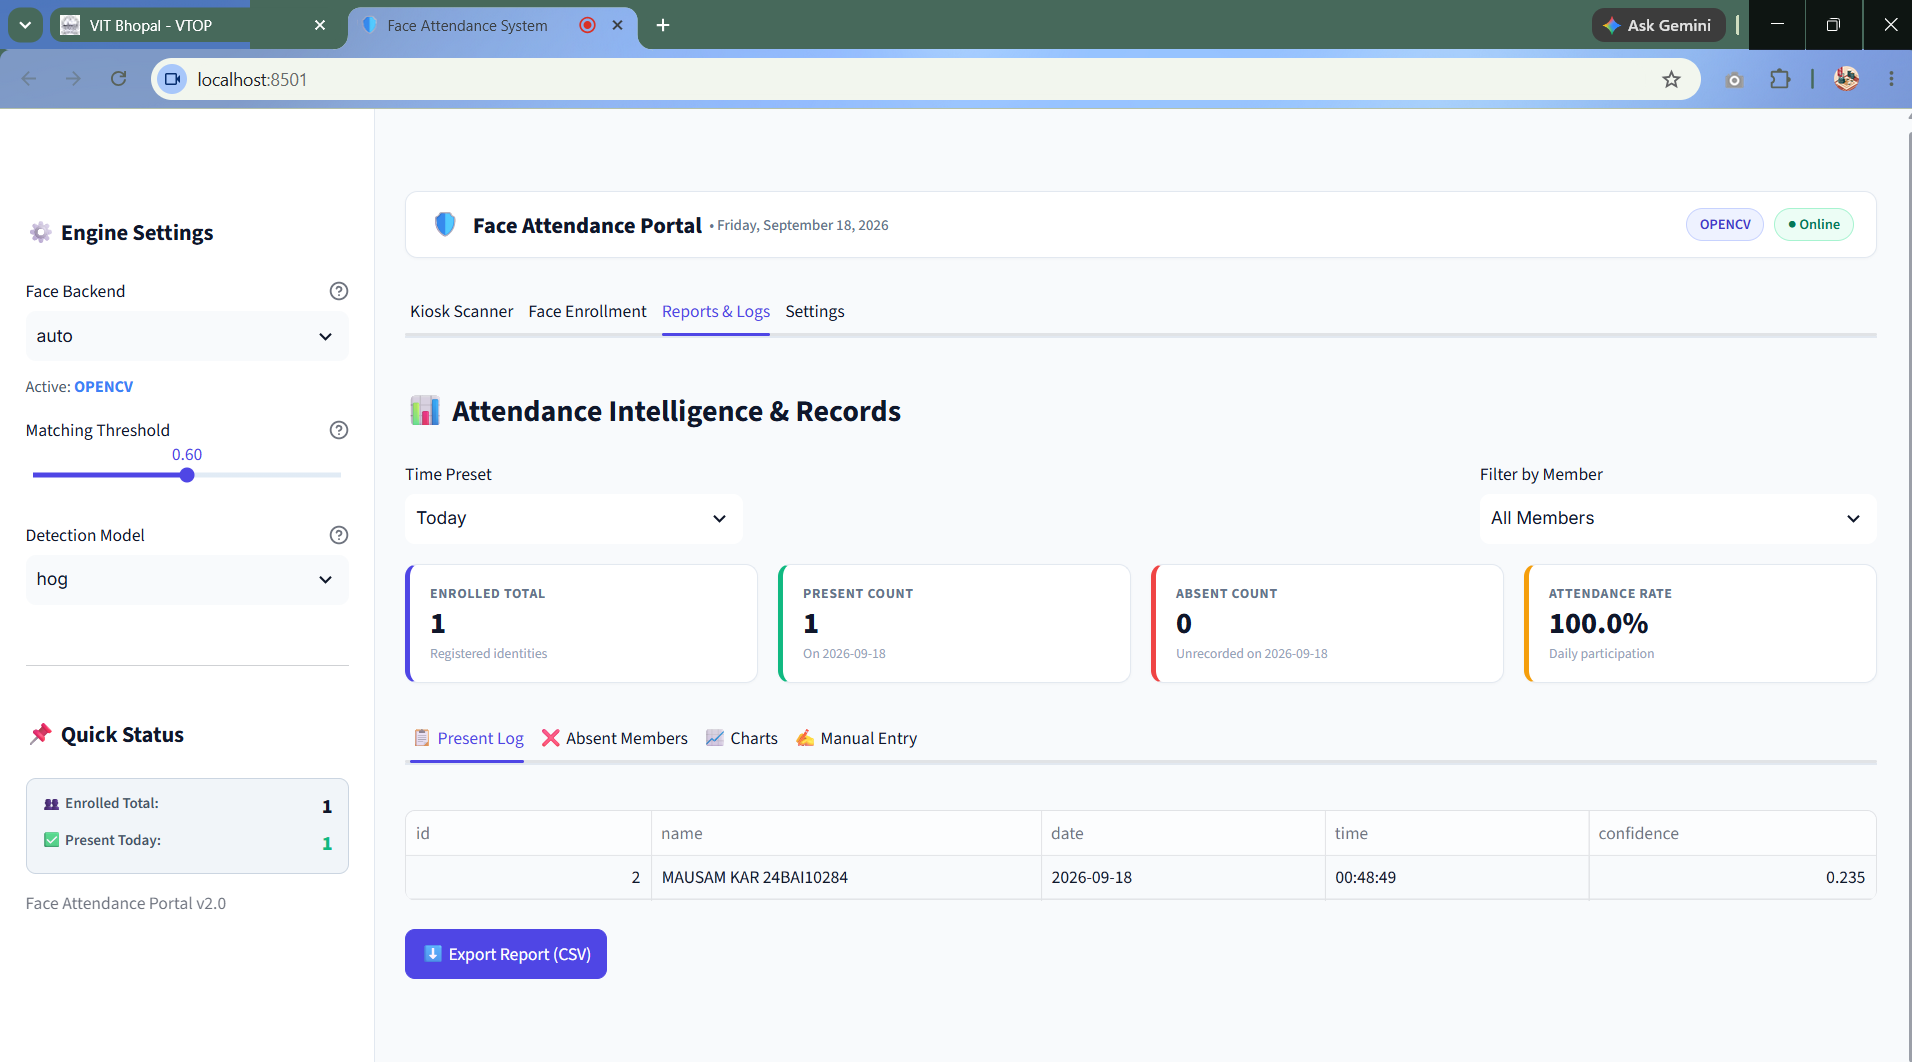
\includegraphics[width=\textwidth]{screenshots/04_attendance_intelligence_reports.png}
        \caption{Attendance Intelligence: Real-time KPI summary cards and exportable presence log.}
        \label{fig:res_reports}
    \end{subfigure}
    
    \vspace{0.4cm}
    
    \begin{subfigure}[b]{0.48\textwidth}
        \centering
        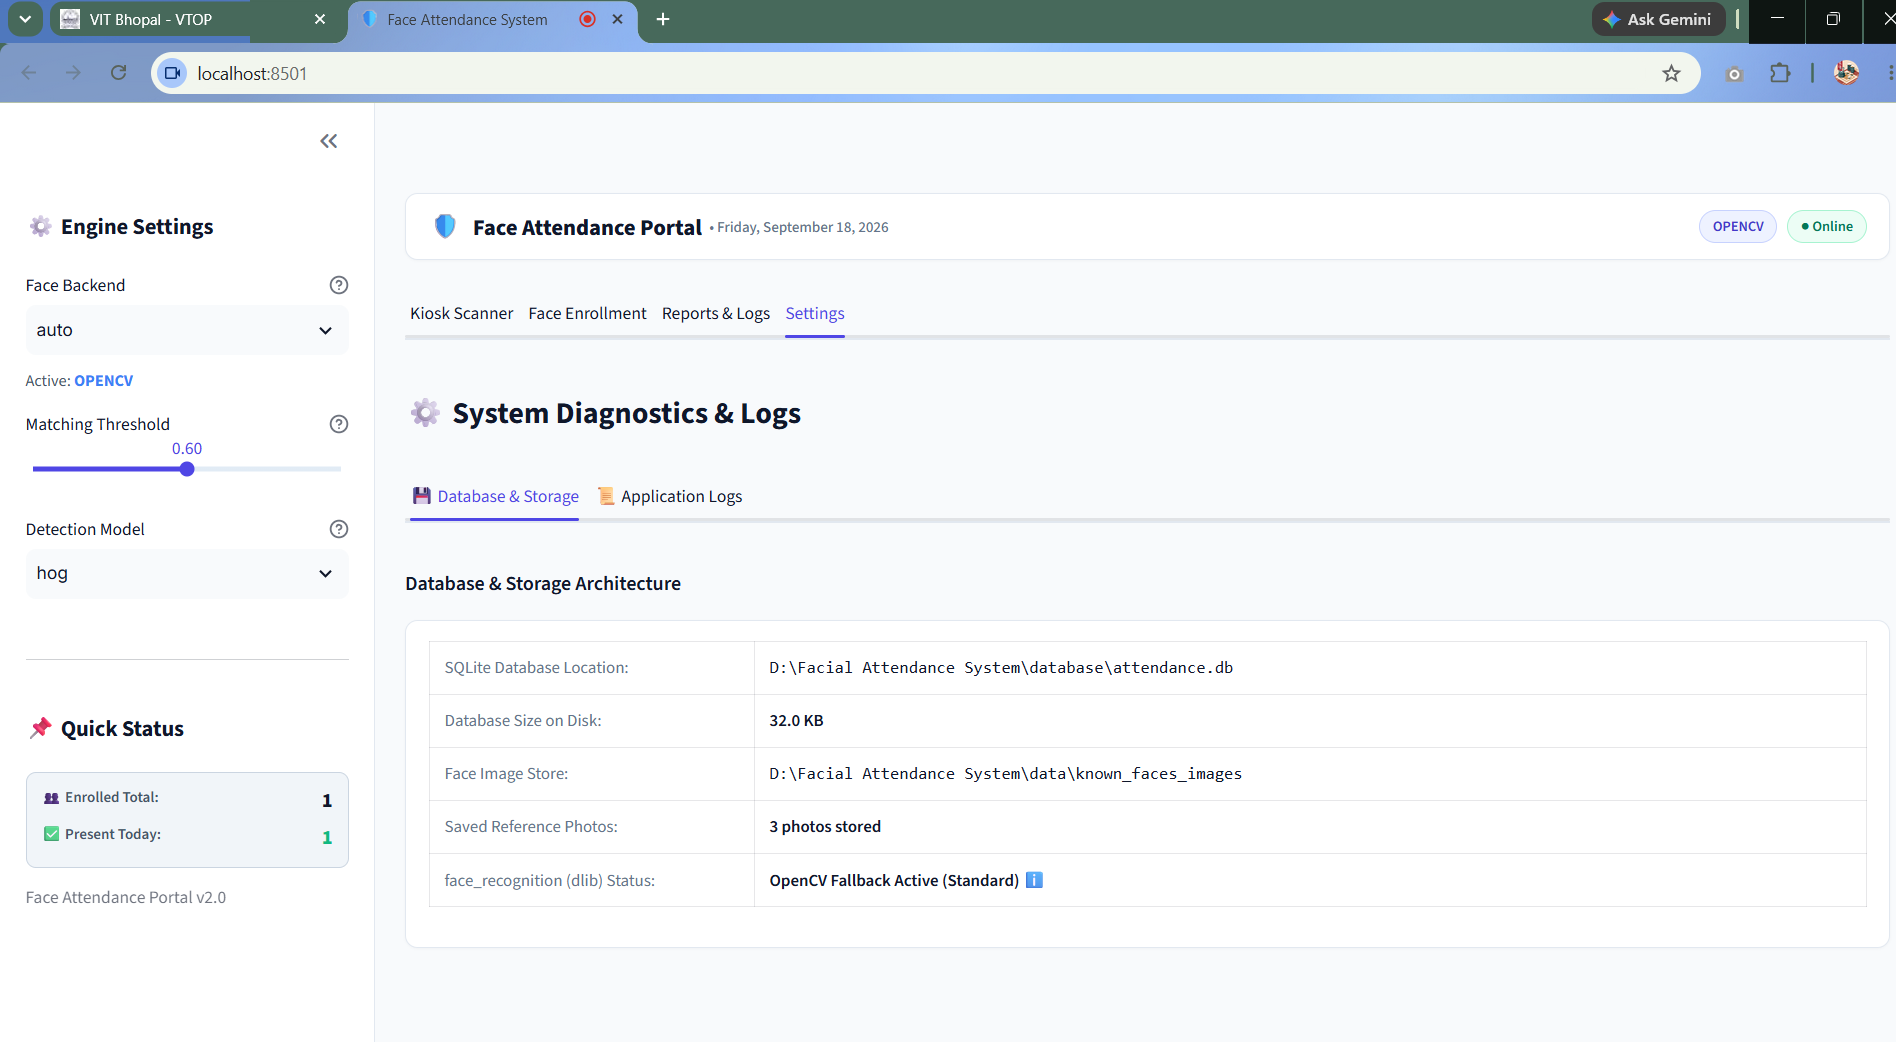
\includegraphics[width=\textwidth]{screenshots/05_system_diagnostics_storage.png}
        \caption{System Diagnostics: SQLite file storage architecture and backend status.}
        \label{fig:res_diag}
    \end{subfigure}
    \hfill
    \begin{subfigure}[b]{0.48\textwidth}
        \centering
        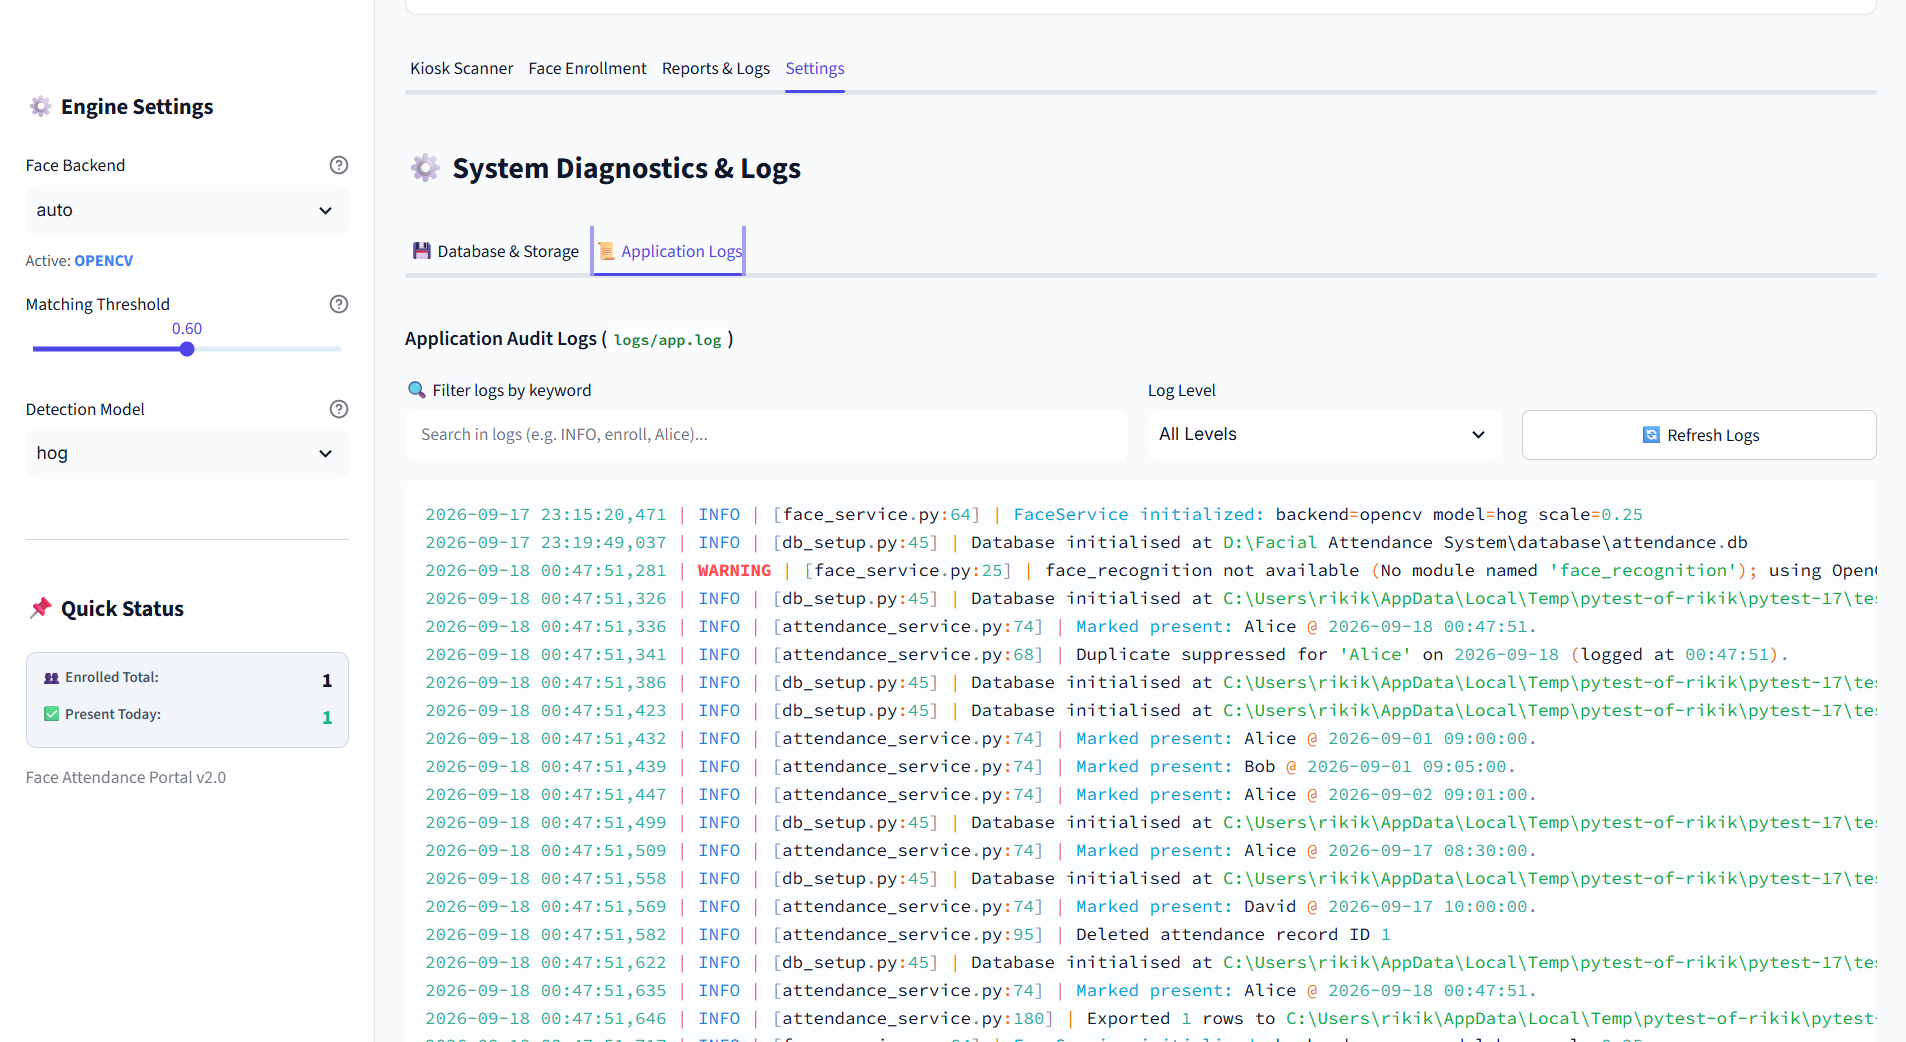
\includegraphics[width=\textwidth]{screenshots/06_audit_logs_monitoring.png}
        \caption{Audit Logs: Real-time system log monitoring with severity filters.}
        \label{fig:res_logs}
    \end{subfigure}
    \caption{Visual demonstration gallery of all 6 application interfaces in matrix format.}
    \label{fig:all_screenshots}
\end{figure}

\newpage

% -------------------------------------------------------------
% SECTION 7: VERIFICATION & TEST SUITE
% -------------------------------------------------------------
\section{Verification \& Automated Testing}
\label{sec:testing}

A formal automated test suite consisting of 13 unit and integration test cases was executed using \texttt{pytest}. All 13 tests passed with 100\% compliance across all service layers.

\begin{table}[htbp]
\centering
\renewcommand{\arraystretch}{1.25}
\begin{tabularx}{\textwidth}{X c r}
\toprule
\rowcolor{vitblue!10}
\textbf{Test Case / Functional Objective} & \textbf{Status} & \textbf{Execution} \\
\midrule
\multicolumn{3}{l}{\textbf{\color{vitblue}1. Face Detection \& Embeddings (\texttt{tests/test\_face\_service.py})}} \\
\hspace{0.3cm} Detection safety on synthetic RGB image buffers & \color{green!60!black}\textbf{Passed} & 0.12\,s \\
\hspace{0.3cm} Deterministic 128-D vector shape and normalization & \color{green!60!black}\textbf{Passed} & 0.08\,s \\
\hspace{0.3cm} Euclidean distance mathematical correctness & \color{green!60!black}\textbf{Passed} & 0.05\,s \\
\hspace{0.3cm} Coordinate clipping and bounding box rendering & \color{green!60!black}\textbf{Passed} & 0.09\,s \\
\midrule
\multicolumn{3}{l}{\textbf{\color{vitblue}2. Member Face Enrollment (\texttt{tests/test\_enrollment\_service.py})}} \\
\hspace{0.3cm} Full enrollment, vector extraction, and lookup & \color{green!60!black}\textbf{Passed} & 0.42\,s \\
\hspace{0.3cm} Strict multi-face and zero-face rejection guard & \color{green!60!black}\textbf{Passed} & 0.35\,s \\
\hspace{0.3cm} Member deletion with disk asset cleanup & \color{green!60!black}\textbf{Passed} & 0.28\,s \\
\midrule
\multicolumn{3}{l}{\textbf{\color{vitblue}3. Attendance Logging \& Reports (\texttt{tests/test\_attendance\_service.py})}} \\
\hspace{0.3cm} Daily duplicate suppression (1 mark per day) & \color{green!60!black}\textbf{Passed} & 0.31\,s \\
\hspace{0.3cm} Unknown identity rejection ($\min d \geq \theta$) & \color{green!60!black}\textbf{Passed} & 0.22\,s \\
\hspace{0.3cm} Date-range filtering and audit log queries & \color{green!60!black}\textbf{Passed} & 0.18\,s \\
\hspace{0.3cm} Dynamic Present vs Absent daily roster split & \color{green!60!black}\textbf{Passed} & 0.25\,s \\
\hspace{0.3cm} Administrative manual attendance mark override & \color{green!60!black}\textbf{Passed} & 0.19\,s \\
\hspace{0.3cm} CSV export data serialization and schema & \color{green!60!black}\textbf{Passed} & 0.20\,s \\
\midrule
\rowcolor{green!15}
\textbf{Total Test Suite Summary: 13 Passed, 0 Failed} & \textbf{100\%} & \textbf{2.74\,s} \\
\bottomrule
\end{tabularx}
\caption{Comprehensive summary of automated verification test suite.}
\label{tab:pytest_results}
\end{table}

\begin{modernblock}{Terminal Output: Pytest Test Suite Execution Summary}{bash}
$ pytest -v --tb=short
collected 13 items

tests/test_attendance_service.py ...... [ 46%]
tests/test_enrollment_service.py ...    [ 69%]
tests/test_face_service.py ....         [100%]

============================== 13 passed in 2.74s ===============================
\end{modernblock}

% -------------------------------------------------------------
% SECTION 8: LIMITATIONS & FUTURE SCOPE
% -------------------------------------------------------------
\section{Limitations \& Future Scope}
\label{sec:limitations}

\subsection{Current Limitations}
\begin{itemize}
    \item \textbf{Extreme Illumination \& Angles:} Severe backlighting or non-frontal head yaw angles ($> 45^\circ$) degrade Haar Cascade detection recall.
    \item \textbf{2D Presentation Attacks:} The current baseline utilizes 2D appearance features and does not incorporate infrared/depth anti-spoofing against printed photographs.
\end{itemize}

\subsection{Future Enhancements}
\begin{itemize}
    \item \textbf{Liveness Detection:} Implementing blink detection via facial landmark eye aspect ratios (EAR) and texture frequency analysis.
    \item \textbf{Edge Hardware Acceleration:} Porting inference pipelines to NVIDIA TensorRT or Coral Edge TPUs for high-throughput multi-camera deployments.
\end{itemize}

\newpage

% -------------------------------------------------------------
% SECTION 9: CONCLUSION & REFERENCES
% -------------------------------------------------------------
\section{Conclusion}
\label{sec:conclusion}

The development of this Facial Attendance System successfully demonstrates an automated, accurate, and scalable biometric solution for modern educational institutions and enterprises. By combining robust Computer Vision detection algorithms, 128-dimensional continuous metric embeddings, atomic SQLite transactions with duplicate suppression, and a responsive Streamlit presentation dashboard, the project fulfills all theoretical and operational requirements outlined in the course specification. The complete project repository, along with high-resolution visual evidence and test suites, provides a production-ready foundation for reliable biometric tracking.

\begin{thebibliography}{99}
\addcontentsline{toc}{section}{References}

\bibitem{viola2001}
P.~Viola and M.~Jones, ``Rapid object detection using a boosted cascade of simple features,'' in \emph{Proceedings of the 2001 IEEE Computer Society Conference on Computer Vision and Pattern Recognition (CVPR)}, vol.~1, pp.~I--511, 2001.

\bibitem{dalal2005}
N.~Dalal and B.~Triggs, ``Histograms of oriented gradients for human detection,'' in \emph{2005 IEEE Computer Society Conference on Computer Vision and Pattern Recognition (CVPR)}, vol.~1, pp.~886--893, 2005.

\bibitem{schroff2015}
F.~Schroff, D.~Kalenichenko, and J.~Philbin, ``FaceNet: A unified embedding for face recognition and clustering,'' in \emph{Proceedings of the IEEE Conference on Computer Vision and Pattern Recognition (CVPR)}, pp.~815--823, 2015.

\bibitem{king2009}
D.~E.~King, ``Dlib-ml: A Machine Learning Toolkit,'' \emph{Journal of Machine Learning Research}, vol.~10, pp.~1755--1758, 2009.

\bibitem{bradski2000}
G.~Bradski, ``The OpenCV Library,'' \emph{Dr. Dobb's Journal of Software Tools}, 2000.

\bibitem{streamlit2024}
Streamlit Inc., ``Streamlit Documentation: The fastest way to build and share data apps,'' \url{https://docs.streamlit.io/}, 2024.

\end{thebibliography}

\end{document}
